\documentclass{article}
\usepackage{graphicx} % Required for inserting images

\title{Global Convergence Newton}
\author{Raffael Colonnello, Fynn Gohlke, Benedikt Heuser}
\date{July 2025}

\begin{document}

\maketitle

\section{Introduction}

Newton's method is a popular optimization algorithm that is commonly used to solve optimization
problems. It is a second-order optimization algorithm since it uses second-order information of the
objective function. Newton's method is known to have fast local convergence guarantees for convex
functions. However, the global convergence properties of Newton's method are still an active area of
research. The purpose of this project is to survey and analyze various strategies to achieve global
convergence.

This sentence will be cited by the sources so i can test if bibtex is working properly \cite{hanzely2022damped} 

\section{Background}

\subsection{Classic Newton}

\subsection{Regularized Newton}

In their 2023 article Michenko presents a variation of Newton's method that uses the update rule \cite{mishchenko2023regularized}:

\begin{equation}
  x^{k+1} = x^{k} - ( \nabla^2 f(x^k) + \sqrt{H||\nabla f(x^k)||\bold{I}})^{-1} \nabla f(x^k)
  \label{eq:regularized-newton}
\end{equation}

where $H > 0$ is a constant. The convergence rate of this algorithm is $\mathcal{O}(\frac{1}{k^2})$.

\bibliographystyle{unsrt}
\bibliography{refs}

\begin{figure}
  \begin{center}
    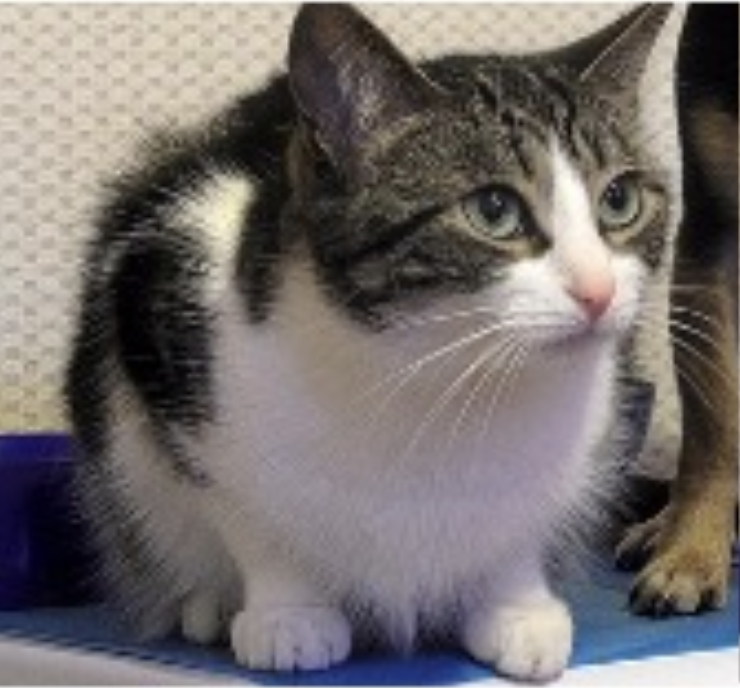
\includegraphics[width=0.5\textwidth]{figures/cat.png}
  \end{center}
  \caption{}\label{fig:}
\end{figure}

\end{document}

